%! TEX root = main.tex
\documentclass[main.tex]{subfiles}
\begin{document}
\section{Einführung in den 3D-Druck}

Das Feld des Additive Manufacturings (AM) entstand bereits 1986 durch die Erfindung des SLA-Prozesses durch Charles Hull. 
Diese revolutionäre Technologie wurde erst im 21. Jahrhundert wirklich realisiert, da diese Methode in jedem Sinne ihrer Zeit vorging. AM und im weiteren Sinne Rapid Prototyping ermöglichen in der Luftfahrt, Medizin, Automobilproduktion, etc. eine schnelle Iteration der Prototypen und veringern damit die Zeit für die Forschung und Entwicklung eines Produktes. 
Zudem ist der Preis von Additive Manufacturing Maschinen stark gesunken in den letzten Jahren, was es sogar Privatpersonen ermöglicht solche Geräte zu besitzen und benutzen. \parencite{BHATIA20231060}

\begin{wrapfigure}{r}{0.4\textwidth}
	
	\copyrightbox{left}{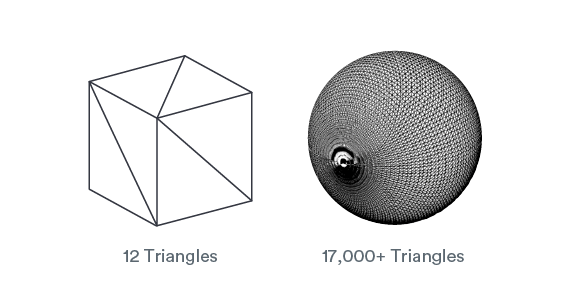
\includegraphics[width=.4\textwidth]{stl_file_1}}{https://www.protolabs.com/media/1022944/pl-dt-may-2021_570x308-02.png}
	\caption{Wiremesh eines Würfels und einer Kugel als STL-Datei}
	\label{img:stl_1}
\end{wrapfigure}
Die Grundlage eines jeden 3D-gedruckten Modells ist immer ein Computer-Assisted-Design-Modell (CAD), welches das gewünschte Teil durch diverse Grundformen wie Würfel und Kugeln darstellt, welche miteinander verbunden und geschnitten werden. Diese Modelle werden nun in Standard-Tesselation-Language-Datei (STL) konvertiert. Eine STL-Datei stellt das Modell als eine Punktwolke dar, wobei immer 3 Punkte ein Dreieck bilden. Dieses Konzept ist sehr effizient darin, Rechtecke darzustellen, da diese nur aus 2 Dreiecken bestehen. Wenn jedoch eine Kugel benötigt wird, ist eine STL-Datei nicht effizient, da immer etwas Ungenauigkeit durch dieses Kozept eingeführt wird. \ref{img:stl_1}
	
\end{document}
